\section{Aim}

The rule based bids do not take into consideration the fact that a lot of time, increasing bids is not the best way to get better performance. A number of times, it happens that a target performs the best (in terms of ACOS) in a range of bids. This range is called the optimum bid range. This chapter describes the method to find the optimum bid range for a target.

\section{Assumptions}

A number of assumptions are inherent in the method described in this chapter. These assumptions are listed below:

\begin{enumerate}
    \item The optimal bid of the targets is independent of the date. That is, if the targets has been performing best 5 INR during the last two months, it will continue to perform best at 5 INR in the future as well.
    \item The optimal bid does not depend on the spend or sales of a single day but only on the average spend and sales of the target.
    \item Data for last 60 days is available.
\end{enumerate}

\section{Algorithm}

The algorithm uses the last 60 days of data. The idea is to use the data for last 60 days to calculate a mean and standard deviation of the bids that minimize or maximize the required metrics. Later, we can use these two values to create the bid range.

\subsection{Metrics Available in the Algorithm}

The algorithm supports the following metrics:

\begin{enumerate}
    \item \textbf{ACOS}: Minimize the ACOS.
    \item \textbf{clicks}: Maximize the spend.
    \item \textbf{Sales}: Maximize the sales.
    \item \textbf{Impressions}: Maximize the impressions.
\end{enumerate}

Other metrics can be added easily. Here is the algorithm:

\subsection{Remove the Outliers}

The first step involves removing the outliers. This is necessary because the outliers can skew the results. The outliers are removed from both the end, that is, the items that are very low from the minimum and very high from the maximum are removed. The outliers are removed using the quartiles. The method is as follows:

\begin{enumerate}
    \item Start with an epsilon value of, say 0.2. Call it \(\epsilon\).
    \item This value is used to remove the top and bottom \(\epsilon\) fraction of the data.
    \item If less than 3 items are left, then decrease the value of \(\epsilon\) by 0.05 and repeat the process until either 3 items are left or \(\epsilon\) becomes 0.05.
\end{enumerate}

\begin{outline}
    At least three items are required to calculate the optimum bid range because we want to determine the mean and standard deviation of the data. If there are less than three items, then the mean and standard deviation will not be good.
\end{outline}


\subsection{Get The Best Values}

Next, we take 10 or 20\% of the items with the best metrics. For example, if the metrics is sales, we will take the top 10 or 20\% of the items with the highest sales and get the bids corresponding the items. We will use these bids to calculate the mean and standard deviation. The algorithm also supports getting the minimum and maximum values instead of the mean and standard deviation. This is done by setting the \texttt{data\_return\_type} parameter to \texttt{min\_max}.

Here is a visualization of the algorithm:

\begin{figure}[ht]
    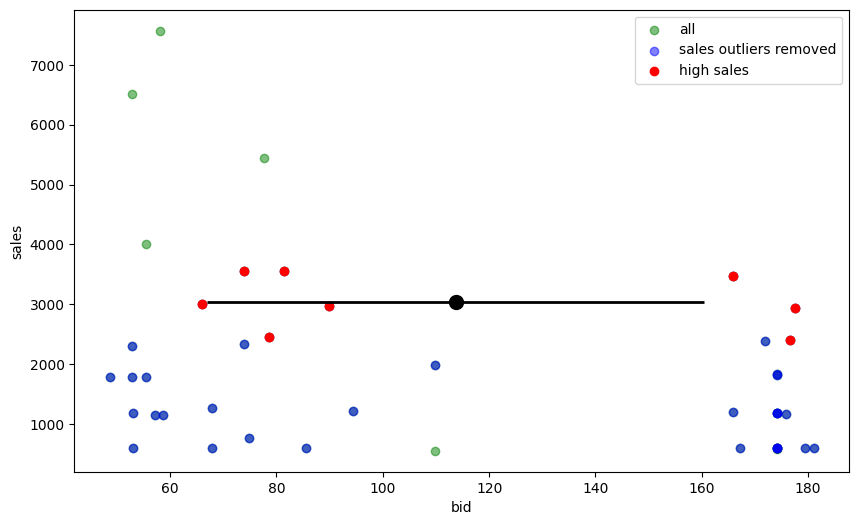
\includegraphics[width=\textwidth, height=0.6\textwidth]{images/part2/bid_range_0.png}
    \centering
    \caption{The Algorithm to Get the Best Values}
\end{figure}

\section{Effect of Parameters}

\subsection{Effect of Outliers}

The following figure shows the effect of outliers on the bid range. The outliers are removed using the method described above. The figure shows that the outliers have a significant effect on the bid range. The bid range is much higher when the outliers are not removed.

\begin{figure}[ht]
    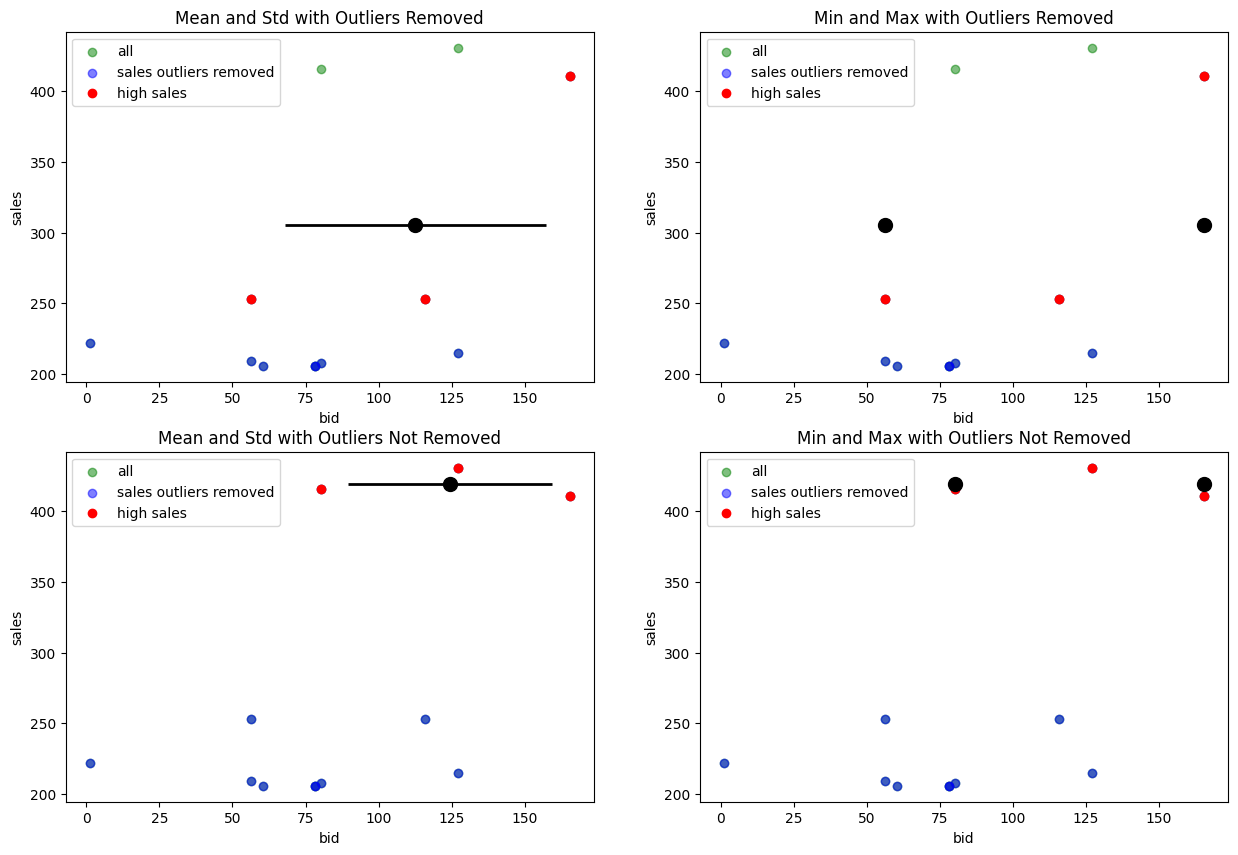
\includegraphics[width=\textwidth, height=0.6\textwidth]{images/part2/bid_range_1.png}
    \centering
    \caption{Effect of Outliers on the Bid Range}
\end{figure}

\subsection{Effect of Metrics}

The bid range changes based on what metrics is used. The following figure shows the effect of metrics on the bid range. The bid range changes significantly based on the metrics.

\begin{figure}[ht]
    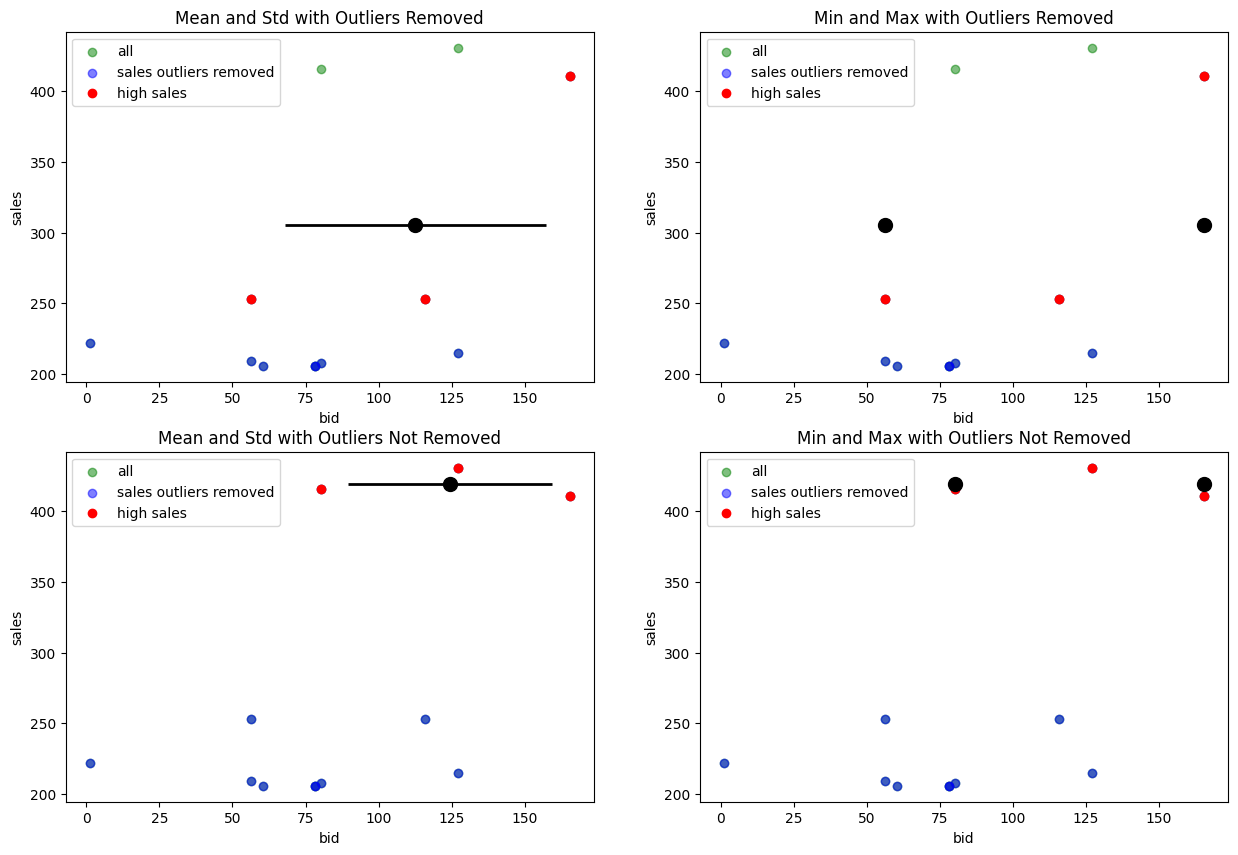
\includegraphics[width=\textwidth, height=0.6\textwidth]{images/part2/bid_range_1.png}
    \centering
    \caption{Effect of Metrics}
\end{figure}


\section{BidRange Class}

The BidRange class is designed to predict a bid range based on a specified column name. The column name can be sales, clicks, impressions, or acos. The class is initialized with a pandas DataFrame, a column name to use, and an optional logger. If no logger is provided, a new one is created.

\begin{lstlisting}[language=Python]
class BidRange:
    def __init__(self, data, column_to_get="bid", logger=None):
        # Code implementation
\end{lstlisting}

\subsection{\_remove\_outliers Method}

The \_remove\_outliers method removes outliers from an array based on a specified quantile.

\begin{lstlisting}[language=Python]
def _remove_outliers(self, array, eps=0.1, verbose=False):
    # Code implementation
\end{lstlisting}

\subsection{\_get\_bids\_for\_top\_value Method}

The \_get\_bids\_for\_top\_value method returns the ids of values that are within a certain quantile range.

\begin{lstlisting}[language=Python]
def _get_bids_for_top_value(self, array, eps=0.80, verbose=False):
    # Code implementation
\end{lstlisting}

\subsection{\_get\_bids\_for\_bottom\_value Method}

The \_get\_bids\_for\_bottom\_value method returns the ids of values that are within a certain quantile range.

\begin{lstlisting}[language=Python]
def _get_bids_for_bottom_value(self, array, eps=0.10, verbose=False):
    # Code implementation
\end{lstlisting}

\subsection{visualize\_one Method}

The visualize\_one method visualizes the bid range for a single targeting id.

\begin{lstlisting}[language=Python]
def visualize_one(self, sample_id, ax=None, legend=False, column_name="sales", strategy="maximize", data_return_type="mean_std", remove_outliers=True):
    # Code implementation
\end{lstlisting}

\subsection{\_bid\_range\_one Method}

The \_bid\_range\_one method calculates the mean and standard deviation of the bids for a single targeting id based on a specified column name and strategy.

\begin{lstlisting}[language=Python]
def _bid_range_one(self, targeting_id, column_name="sales", strategy="maximize", min_rows_to_use=3, min_rows_breach_behaviour="warn", data_return_type="mean_std", remove_outliers=True):
    # Code implementation
\end{lstlisting}

\subsection{\_bid\_range Method}

The \_bid\_range method calculates the mean and standard deviation of the bids for all column names and strategies.

\begin{lstlisting}[language=Python]
def _bid_range(self, targeting_id, min_rows_to_use=3, min_rows_breach_behaviour="leave", data_return_type="mean_std", remove_outliers=True):
    # Code implementation
\end{lstlisting}

\subsection{bid\_range\_all Method}

The bid\_range\_all method applies the \_bid\_range method to all targeting ids in the DataFrame and returns a DataFrame with the results.

\begin{lstlisting}[language=Python]
def bid_range_all(self, min_rows_to_use=3, min_rows_breach_behaviour="leave", data_return_type="mean_std", remove_outliers=True):
    # Code implementation
\end{lstlisting}
